\section{\name: a Secure Embedded OS}
\label{sec:os}

\name is an operating system  designed for embedded platforms
with multiple processors running multiple concurrent applications.
\name's design centers around protection, both from potentially
malicious applications and from device drivers. \name uses three
mechanisms to protect different components of the operating
system. First, the kernel and device drivers are written in Rust~\cite{rust}, 
a systems programming language that provides compile-time memory safety, 
type safety and
strict aliasing. \name uses Rust to protect the kernel (e.g. the
scheduler and hardware abstraction layer) from platform specific
device drivers as well as isolate device drivers from each other. 
Second, \name uses memory protection units
 to isolate applications from each other and
the kernel. Finally, when available, \name uses multiple microcontrollers to
protect applications with timing concerns against starvation or leaking
information through side-channels. The remainder of this section gives an
overview of the \name architecture, focusing on how the kernel uses the
MPU for protection while simultaneously giving applications direct access
to hardware.

\subsection{Architecture}
\label{sec:os-arch}

\begin{figure}
 \centering
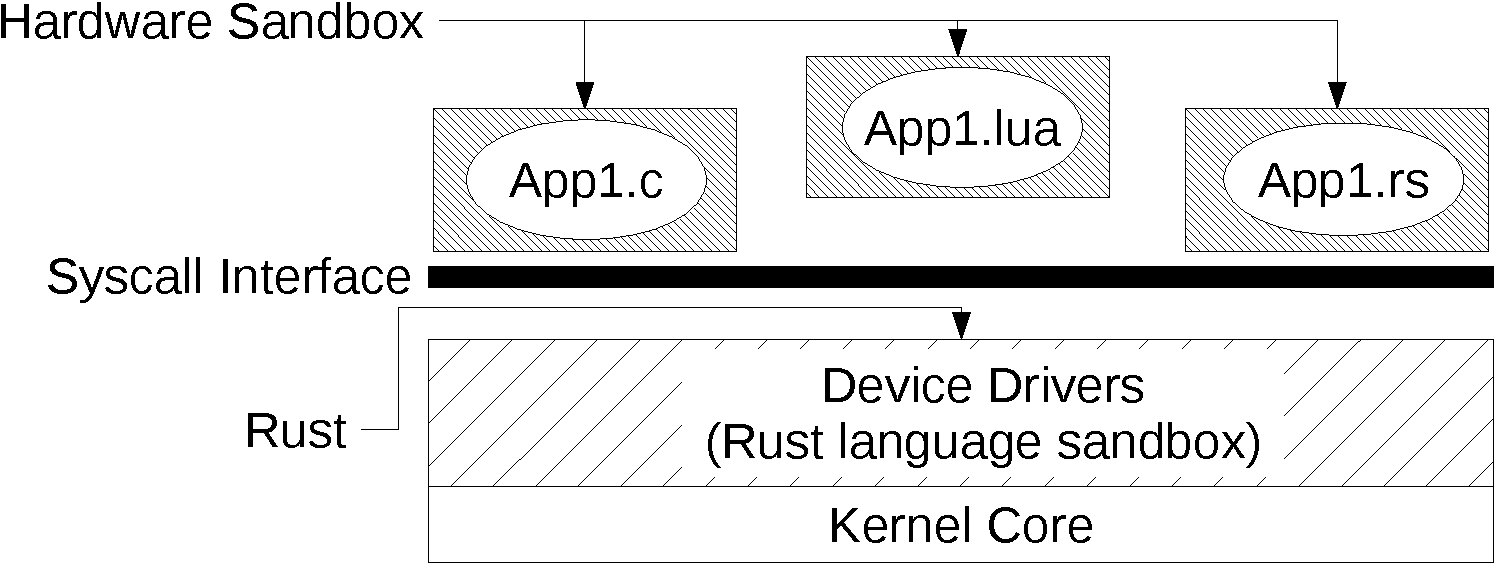
\includegraphics[width=1\columnwidth]{img/architecture-crop}
\caption{\name is written in Rust, a type-safe, memory-safe systems language.
The \name kernel's core has full access to the underlying hardware. Device
drivers run with no hardware protection, but within a language sandbox that
constrains their access to hardware. Applications are sandboxed using the MPU, a
hardware memory protection mechanism, and can be written in any language (e.g.
C, Rust, or even a scripting language like Lua).}
\label{fig:architecture}
\end{figure}

% Definitions:
%  Tock core -- the kernel code shipped and provided with base Tock
%  Tock kernel -- the final compiled kernel, including core and drivers

The \name kernel has complete system access, including arbitrary memory
access and interrupt control. Device drivers are compiled into the kernel and
run with the same \emph{hardware} privileges but inside a
\emph{language-level} sandbox. This sandbox statically enforces that device
drivers only use kernel hardware interfaces, limits dynamic memory
allocation to load time, and prevents uncoordinated access of underlying
hardware resources.

Applications are separated from the kernel by a syscall ABI and can be
written in any language that can interface with the ABI. 
Applications have an execution stack, an application memory
heap, and a kernel memory heap. Kernel (and driver) dynamic allocations take
place in the application memory space, thus charging applications for buffers
the kernel creates on their behalf and ensuring that an out-of-memory
condition terminates the application and does not cause a kernel error. 
The kernel uses the MPU to protect the application-level kernel memory heap
from application access.

The ABI can provide direct access to system hardware resources. If an 
application requires direct access, it can request it from the kernel.
If granted, the kernel uses the MPU to make the memory mapped I/O region
of specific peripherals accessible to the application. Because processors
such as the Cortex M support access permissions on as fine grained boundaries
as 32 bytes, the kernel can expose one port of GPIO pins but not others.
Enabling this kind of access safely requires that kernel-controlled
peripherals be connected only to GPIO ports that cannot be exposed.

%% Brad: not sure what this paragraph contributes to the paper, particularly
%% in this section. I think the contents of this should be discussed in the sections above, if
%% at all.
% Scheduling in \name is an open question, particularly if it aims to capitalize
% on multi-MCU systems. Some assignments are clearer, a communication task
% should likely run on the same core as the radio controller. Applications
% that require hard real-time could run on a dedicated core with a real-time
% scheduler, but what if another core is not available? Technology such as
% TrustZone~\cite{trustzone}, a secure processing mode on the same physical
% core, provides protection for sensitive data, but not from side-channel
% attacks such as timing.


% TrustZone is interesting, but currently only available on Cortex-A's, not
% clear if there's any intention of bringing to M's. Maybe this though belongs
% more in the HW section earlier?

\subsection{Execution Model}

When a device powers on or resets, \name loads each application by allocating a
fixed sized memory region for it's stack, heap and data
(\Cref{sec:arch:memory-design}), configuring the MPU, switching to an
unprivileged execution mode and jumping to the application's {\tt init}
function. While executing, the application can request resources (e.g. access to
the \emph{TRNG} memory mapped registers), register for callbacks to events (e.g. a
timer or sensor interrupt) and issue commands (e.g. send a packet over the
radio). Applications run in a single thread and will not be interrupted by event
callbacks until either invoking the {\tt wait} system call, or returning from
{\tt init} (which is an implicit {\tt wait}). Once an application has issued the
{\tt wait} system call, the kernel suspends it until a relevant event has fired,
and a callback can be invoked. Finally, the kernel invokes callbacks by pushing
an additional stack frame onto the application's stack and jumping to the
callback function. Thus, when a callback function returns, execution is resumed
where the {\tt wait} system call was invoked.


% \subsection{The Cortex-M MPU}
%
% The Cortex-M MPU allows the kernel to defined eight memory regions. Each memory
% region may be sized between 32 bytes and 4GB, in 32 byte increments and has
% protection bits for read, write and execute. Regions may overlap, in which case
% the memory region with the highest number ``wins''. In addition, regions of at
% least 256 bytes can be divided into eight equal sized subregions, which can
% either be turned on---in which case they inheret the parent region's protection
% bits---or turned off---in which case the parent's protection bits do not apply.
% As a result, the operating system can control access to up to 64 concurrently
% active regions. Finally, memory regions and protection bits can be changed
% during exection, for example while context switching between applications.

\subsection{\name Memory Design in Detail}
\label{sec:arch:memory-design}

One major challenge in \name is defining a memory management design
that allows untrusted application code 
to interact with a type-safe Rust kernel, for the kernel to be able to
issue event upcalls to the application, for device driver isolation, and 
for applications to directly
access hardware. To achieve this
\name defines four types of memory regions: code regions, 
memory-mapped I/O regions,
kernel stack and static data regions and application regions.
\Cref{fig:memory-layout} shows these regions and their access rules from
an application.

\begin{figure}
 \centering
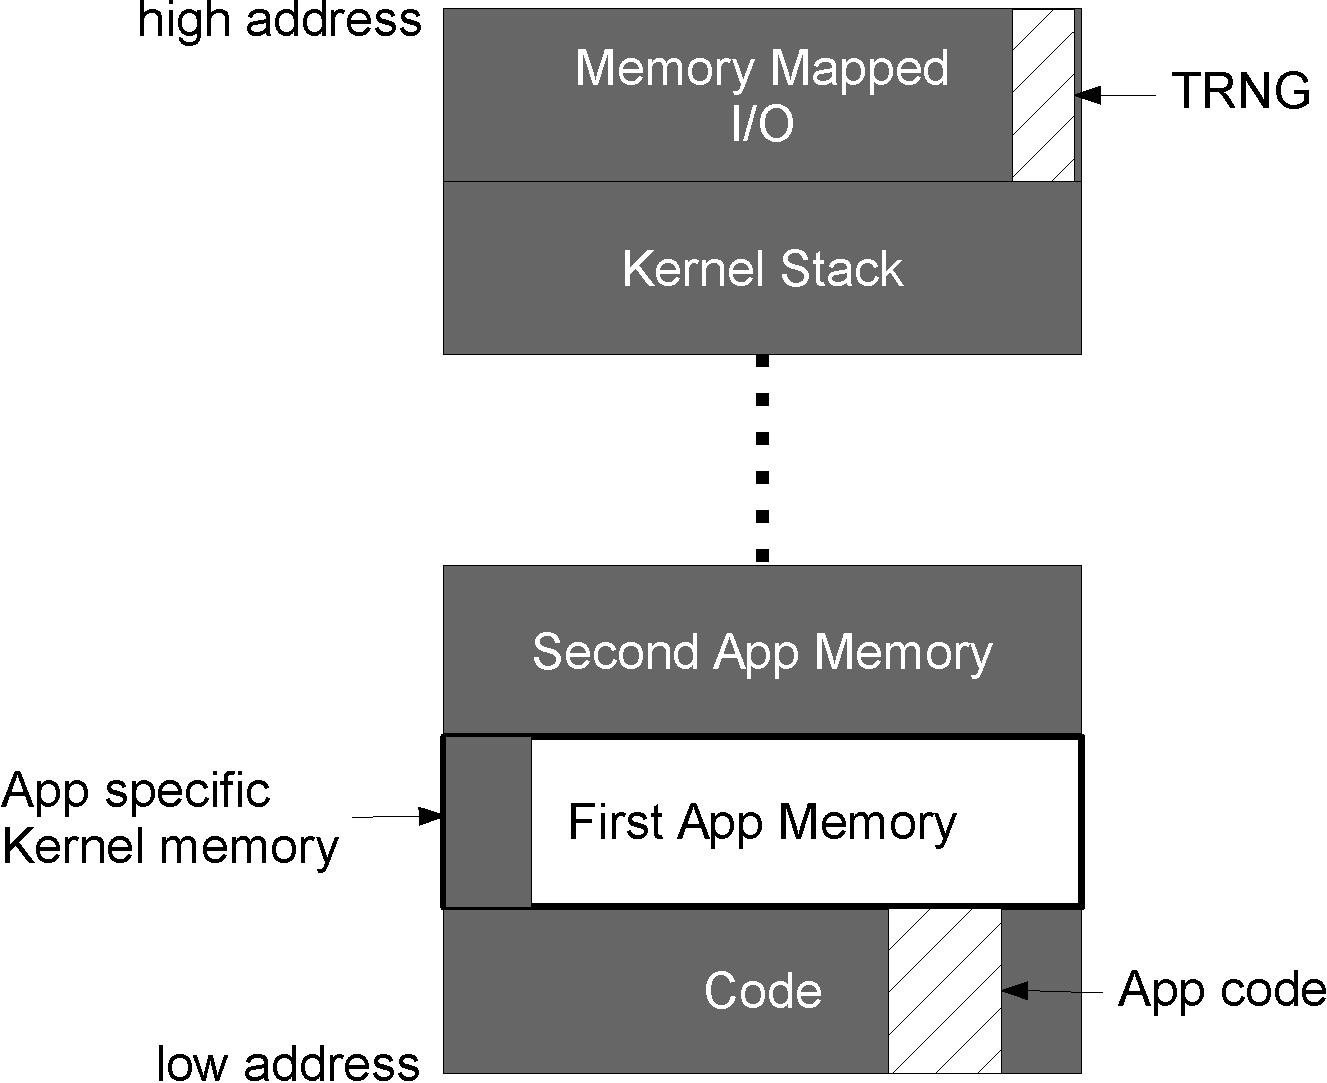
\includegraphics[width=1\columnwidth]{img/memory-layout-crop}
\caption{Memory layout and access permissions while executing an application.
\name lays out memory into four types of regions: code, memory mapped I/O,
application memory and the kernel stack. Greyed regions are marked unreadable
and unwritable, while hatched regions are read-only. The application memory
contains a subregion used by the kernel for application-specific kernel data
structures and is thus inaccessible to the application. Conversely, some
hardware registers are exposed directly to applications by marking them
read-only.}
 \label{fig:memory-layout}
\end{figure}



{\bf Code.}
A code region contains kernel and application code. While an application is
executing code, it only has read and instruction fetch access to its own code
segment. An application cannot write to its own code section because typically
the code is backed by internal flash, which has limited write cycles.

{\bf Memory-Mapped I/O.}
Hardware registers are typically located in a single, continuous region of the
memory space.\footnote{The location of hardware memory registers and flash is
determined by the chip manufacturer, however, chips typically place flash at
the bottom of memory, followed by RAM, and peripheral memory registers towards
the top of memory.} \name may provide read-only or read-write access over small
ranges of memory registers to applications, bypassing the kernel for direct
hardware access. For example, our development platform uses the Atmel SAM4L
Cortex-M4~\cite{sam4l} which provides a true random number generator (TRNG)
peripheral. \name exposes random numbers directly to applications by allowing
read-only access to the TRNG registers.

{\bf Kernel Stack and Static Data.}
These regions include all kernel and device driver memory, including local
variables. The MPU restricts any application-level access to this memory
section.

{\bf Application Memory.}
\name allocates a continuous, fixed size region for each application.
Application memory and the kernel stack grow towards each other to balance
application count with kernel stack size. If the kernel stack grows too large,
\name terminates the application whose memory region is closest to the kernel
stack. Thus, applications with higher priority should be allocated memory
regions at lower memory addresses. We intend to explore an alternate strategy of
allocating application memory from a shared heap using the high granularity of
the MPU.  This would trade-off a simpler process for reclaiming stack space
for better support of heterogeneously sized applications.


Most of an
application's memory is
used for its stack, static variables, and heap. However,
the kernel may also ``borrow'' memory from the top of an application's memory
region for application-specific kernel data structures. This region, which may
change in size,
%is \emph{inside} the application's memory space, but
is marked
as read and write protected when the application is running. This allows the
kernel and device drivers to allocate memory dynamically in response to an
application without
potentially causing an out-of-memory kernel error and while
% sacrificing the reliability of never dynamically
% allocating in the kernel itself and while
maintaining the integrity and
confidentiality of shared kernel data structures. As an example, when an
application registers a callback for a timer, the timer device driver
allocates a new link node for the callback in the application's memory.
% adds the
% request to its list of pending timers by allocating the new list node in the
% application's memory.
Since the link includes forward and backward list
pointers, it is imperative that, despite being in the application's memory,
this link's integrity be maintained. Moreover, the values of the links might
leak information about other applications.

